\section{Validation}\label{sec:validation}
% Objective: What was checked before any note was priced, including the one honest failure and why it is a property of the SPX option market.

A note's value is not observable, so nothing downstream of the pricing engine
can be checked against a market. Everything upstream can be, and is, because a
model that cannot return the instruments it was calibrated to has no claim on
the instrument it was built for. This section reports those checks in the order
the pipeline runs them, including the one that does not pass.

\subsection{Forwards and discount factors}

Each slice's forward comes from a put-call parity regression across
near-the-money strikes. The direct check is how well the fitted forward agrees
with the one the quotes imply, and the maximum relative error across expiries
is 1.6, 1.9 and 4.4 basis points on the three cash indices, 8.0 on the fund
standing in for the Dow and 16.7 on the semiconductor ETF. The two largest are
the two exchange-traded funds, for the reason \S\ref{sec:data} gives: their
options are American, parity is an identity only under European exercise, and
the discount factor is therefore pinned to the Treasury curve rather than
fitted.

Where the discount factor is fitted, it is worth reading as a diagnostic in its
own right. The implied zero rates run from 3.73 to 5.47 per cent and rise with
maturity, against a Treasury curve near 4.3 per cent over the same horizon. The
short end is noisy, which is expected when the regression has a few weeks of
time value to work with. The long end is not noise: index options embed a
financing rate that sits above Treasuries, and the fit recovers it. That rate
enters the forward, and so the diffusion, but not the discounting of the note's
cashflows, which is a separate curve and the object \S\ref{sec:results} solves
for.

\subsection{The arbitrage audit}

Every fitted slice is checked on its own grid for both conditions of
\S\ref{sec:method}. Across all five surfaces and their 68 slices there are zero
butterfly failures and zero calendar failures. The minimum of $g(\logm)$ is
positive on every surface, at its tightest 0.0057 on the S\&P 500, and the
implied risk-neutral density is positive everywhere.

The calendar diagnostic is the more informative of the two. On three of the
five surfaces the minimum gap between adjacent total-variance curves sits at
the solver's tolerance, around $10^{-6}$, which means the constraint is binding
rather than slack: those slices were refitted against it, and without the
constraint the surface would have violated it. On the other two the gap is
three orders of magnitude larger and the condition holds on its own. Reporting
the audit as a pass alone would hide that difference.

\subsection{The repricing gate}

% Generated by scripts/make_paper_tables.py from the frozen results.
% Do not edit by hand; the next build overwrites it.
\begin{table}[tbp]
\centering
\caption{Repricing error against quoted bid-ask width, by surface, in implied volatility points}
\label{tab:validation}
\small
\begin{tabular}{l r r r r r}
\toprule
Surface & Options & Inside spread (\%) & Median error & Median spread & Error/spread \\
\midrule
DJX & 518 & 96.3 & 0.067 & 0.928 & 0.07 \\
NDX & 1,074 & 98.6 & 0.111 & 0.561 & 0.20 \\
RUT & 845 & 96.0 & 0.097 & 0.368 & 0.26 \\
SMH & 921 & 99.5 & 0.173 & 2.157 & 0.08 \\
SPX & 2,378 & 46.3 & 0.131 & 0.079 & 1.67 \\
\bottomrule
\end{tabular}
\notetext{\textit{Notes:} Every option used in the calibration is repriced through the local-volatility engine and the result converted back to implied volatility, so the error is in the units the market quotes. \textit{Inside spread} is the share of repriced options falling within the quoted bid-ask. The final column is the median error divided by the median quoted bid-ask width. Error is measured from the mid and the quoted band runs half a width either side of it, so a ratio below one half puts the model inside the band the market itself prices in. Four surfaces return 0.26 or better; the SPX surface returns 1.67, on a quoted width 4.7 times narrower than the next tightest here, which \S\ref{sec:validation} attributes to that market's liquidity rather than to the fit. Source: \texttt{src/vol/reprice\_check.py}.}
\end{table}


The gate is whether the local-volatility engine, built from a surface, returns
the prices of the vanilla options that surface was fitted to. Each option used
in calibration is repriced through the full Monte Carlo machinery and the
result converted back to implied volatility, so the error is in the units the
market quotes rather than in dollars, where it would be dominated by the level
of whichever index it came from. Table~\ref{tab:validation} reports it.

An error is only large or small relative to the price uncertainty of the market
it came from, so the comparison is against the quoted bid-ask width rather than
against zero. Error is measured from the mid and the quoted band runs half a
width either side, so a ratio below one half puts the model inside the band the
market itself prices. Four of the five surfaces clear that comfortably, at
0.07, 0.08, 0.20 and 0.26. Between 96.0 and 99.5 per cent of their repriced
options land inside the quoted bid-ask outright.

Figure~\ref{fig:smile} shows what that looks like for six S\&P 500 expiries,
with the per-slice fit error in basis points. The fits track the quoted mids
through the body of the smile and part company in the upper wing on two of the
panels, where the quotes thin out. The last panel is the longest listed
expiry at 5.20 years, fitted from ten quoted volatility points against 49 on
the expiry a year before it. Nothing about the extrapolation discussed in
\S\ref{sec:method} shows up as error here, because by that maturity there is
very little left to be in error against.

\subsection{The surface that does not pass}

The S\&P 500 surface returns a ratio of 1.67, and 46.3 per cent of its repriced
options fall inside the quoted bid-ask against 96 per cent or better everywhere
else. Taken at face value that is the worst-fitted surface in the study, and it
belongs to the most liquid index option market in the world, which should be
reason enough to look at the denominator before accepting the verdict.

Its absolute error is 0.131 volatility points. That is the second largest of
the five, sitting between the Nasdaq-100 at 0.111 and the semiconductor ETF at
0.173, and inside the range the other four span. What distinguishes it is the
width it is divided by. The median quoted bid-ask on the S\&P 500 slices is
0.079 volatility points, against 0.368 on the next tightest surface and 2.157
on the widest. The S\&P 500 market quotes roughly four and a half times tighter
than anything else in the sample, so a fit that is unremarkable in absolute
terms fails a test scaled to that market's own precision.

Two readings are available and the data does not fully separate them. Either
the calibration is genuinely less accurate on this surface than the absolute
error suggests, or the test is asking a surface fitted from end-of-day quotes
to reproduce intraday-tight spreads that no daily snapshot could support. The
second is more consistent with the evidence, since the absolute error is
ordinary and the arbitrage audit on this surface is clean. It is reported
either way, because a validation section that only contains passes is not
reporting a validation.

What follows from it for the results is bounded. The S\&P 500 appears as a leg
in five of the six notes, so if this surface carries error the error is
widespread. But the direction is not determined: a vol fit slightly off in
either direction moves a worst-of value in the opposite direction to the
cheapest leg, and \S\ref{sec:inputs} shows that a far larger volatility
perturbation than anything suggested here moves the values the wrong way to
explain the gap.

\subsection{The payoff, the matrix and the pipeline}

Three further checks sit outside the surface machinery. Each note's payoff is
tested against scenarios worked by hand, so that a coupon paid on a barrier
touch, a call on the first eligible date and a principal loss through the
trigger each produce the arithmetic they should rather than merely a plausible
number. The correlation estimator is tested on a matrix constructed to be
non-positive-semidefinite, confirming the repair of \citet{Higham2002} fires
and returns a valid matrix rather than failing quietly at the Cholesky step.
And the six term sheets are tested against the preserved filings, so that a
coupon rate or a trigger transcribed into the configuration cannot drift from
the document it came from.

Reproducibility is checked by construction rather than asserted. A fresh copy
of the repository holding only the shipped files recalibrates all five surfaces
from the preserved option chains bit for bit, passes the test suite, and
regenerates the report byte for byte.

\begin{figure}[tbp]
\centering
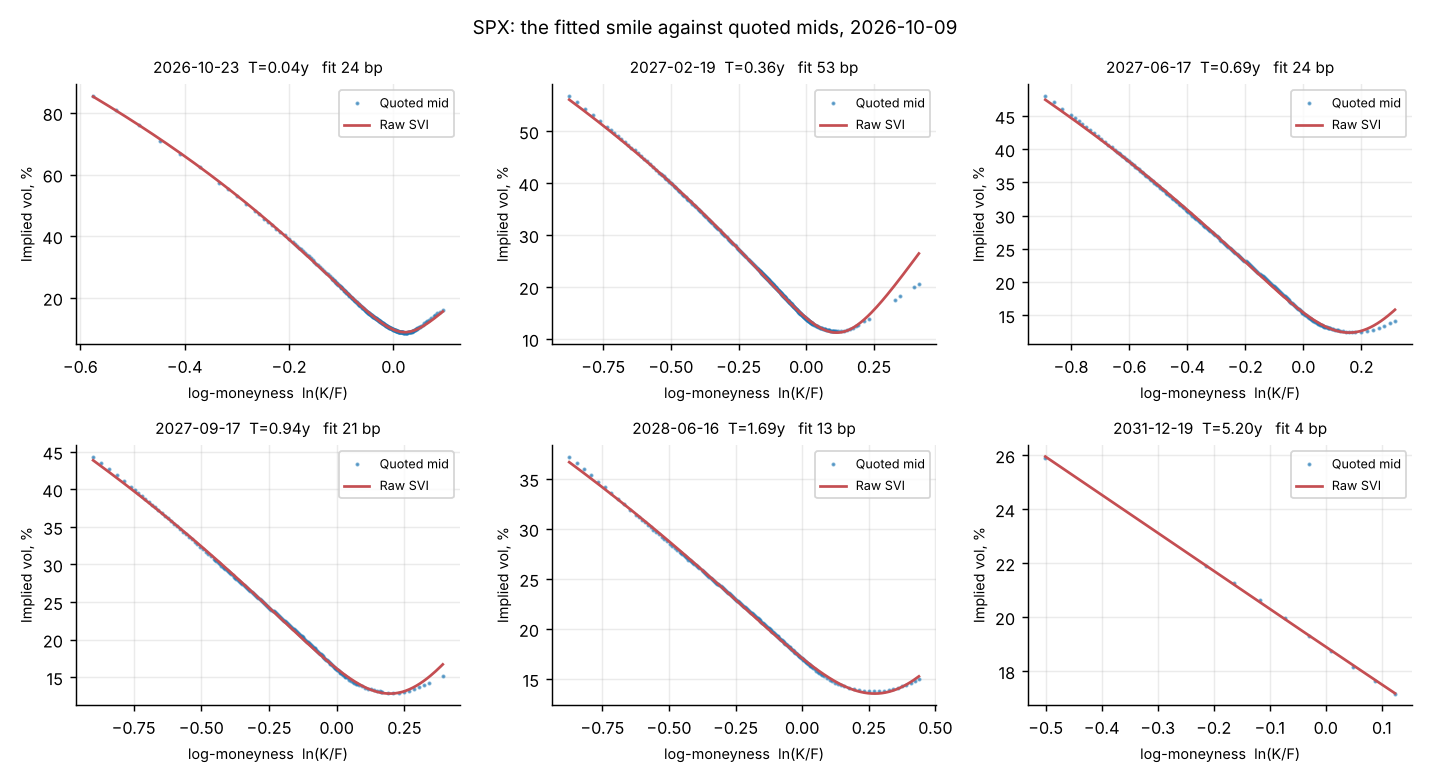
\includegraphics[width=\textwidth]{figures/smile_fits_SPX}
\caption{Fitted S\&P 500 smiles against quoted mids, six expiries from the
9 October 2026 snapshot}
\label{fig:smile}
\notetext{\textit{Notes:} Points are quoted mids, lines the fitted raw SVI
slice. The figure in each panel title is that slice's root-mean-square fit
error in basis points of implied volatility. Panels are ordered by maturity;
the last is the longest listed S\&P 500 expiry at 5.20 years, fitted from ten
quoted volatility points, and each panel plots the quotes falling inside its
own axis range rather than the whole fitted slice. Source:
\texttt{scripts/make\_figures.py}.}
\end{figure}
